\documentclass[aspectratio=169]{beamer}
\usetheme{metropolis}

% =============================================================================
% PACKAGES
% =============================================================================
\usepackage[utf8]{inputenc}
\usepackage[T1]{fontenc}
\usepackage{amsmath,amssymb}
\usepackage{booktabs}
\usepackage{tikz}
\usepackage{fontawesome5}
\usepackage{hyperref}
\usepackage{animate}  % For GIF/frame animation integration
\usepackage{graphicx}
\usetikzlibrary{shapes.geometric, arrows, positioning, calc, backgrounds, decorations.pathmorphing, decorations.markings, arrows.meta, fadings}

% =============================================================================
% ACCESSIBILITY-OPTIMIZED CYBERPUNK COLOR PALETTE (WCAG AA/AAA Compliant)
% =============================================================================
\definecolor{darkbg}{HTML}{0A0E14}        % Primary background
\definecolor{lighttext}{HTML}{E6E6E6}     % Primary text (contrast 14.8:1)
\definecolor{cyanneon}{HTML}{33F5FF}      % Primary accent - AAA compliant
\definecolor{magentaneon}{HTML}{FF3377}   % Secondary accent - AA+ compliant
\definecolor{violetelectric}{HTML}{9D4EDD} % Tertiary accent
\definecolor{subtleglow}{HTML}{1A2332}    % Block backgrounds
\definecolor{goldaccent}{HTML}{FFD700}    % Highlight color

% Semantic colors for diagrams
\definecolor{pathkept}{HTML}{33F5FF}      % Kept edges
\definecolor{pathremoved}{HTML}{FF3377}   % Removed edges
\definecolor{nodeactive}{HTML}{33F5FF}    % Active nodes
\definecolor{nodehub}{HTML}{FF3377}       % Hub nodes
\definecolor{flowcolor}{HTML}{FFD700}     % Electrical flow

% Legacy mappings
\definecolor{distillblue}{HTML}{33F5FF}
\definecolor{distillred}{HTML}{FF3377}
\definecolor{distillgrey}{HTML}{8B95A5}

% =============================================================================
% METROPOLIS THEME OVERRIDES - DARK MODE
% =============================================================================
\setbeamercolor{normal text}{fg=lighttext, bg=darkbg}
\setbeamercolor{alerted text}{fg=magentaneon}
\setbeamercolor{example text}{fg=cyanneon}

% Frame titles
\setbeamercolor{frametitle}{fg=cyanneon, bg=darkbg}
\setbeamercolor{framesubtitle}{fg=lighttext!70}

% Title page
\setbeamercolor{title}{fg=cyanneon}
\setbeamercolor{subtitle}{fg=lighttext!80}
\setbeamercolor{author}{fg=lighttext}
\setbeamercolor{institute}{fg=lighttext!70}
\setbeamercolor{date}{fg=lighttext!70}

% Progress bar
\setbeamercolor{progress bar}{fg=cyanneon, bg=subtleglow}

% Blocks
\setbeamercolor{block title}{fg=darkbg, bg=cyanneon}
\setbeamercolor{block body}{fg=lighttext, bg=subtleglow}
\setbeamercolor{block title example}{fg=lighttext, bg=violetelectric}
\setbeamercolor{block body example}{fg=lighttext, bg=subtleglow}
\setbeamercolor{block title alerted}{fg=lighttext, bg=magentaneon}
\setbeamercolor{block body alerted}{fg=lighttext, bg=subtleglow}

% Structure
\setbeamercolor{structure}{fg=cyanneon}
\setbeamercolor{palette primary}{bg=darkbg, fg=lighttext}
\setbeamercolor{palette secondary}{bg=subtleglow, fg=lighttext}

% Footer
\setbeamercolor{footline}{fg=lighttext!60}

% Table of contents
\setbeamercolor{section in toc}{fg=cyanneon}

% =============================================================================
% FONTS
% =============================================================================
\setbeamerfont{frametitle}{size=\Large, series=\bfseries}
\setbeamerfont{title}{size=\huge, series=\bfseries}
\setbeamerfont{subtitle}{size=\large}
\setbeamerfont{author}{size=\normalsize}
\setbeamerfont{block title}{size=\normalsize, series=\bfseries}

% =============================================================================
% CUSTOM ITEMIZE WITH FONTAWESOME ICONS
% =============================================================================
\setbeamertemplate{itemize item}{\textcolor{cyanneon}{\faAngleRight}}
\setbeamertemplate{itemize subitem}{\textcolor{violetelectric}{\faChevronRight}}
\setbeamertemplate{itemize subsubitem}{\textcolor{magentaneon}{\faMinus}}

% =============================================================================
% CUSTOM FRAME TITLE WITH NEURAL NETWORK BACKGROUND
% =============================================================================
\makeatletter
\setbeamertemplate{frametitle}{%
  \nointerlineskip%
  \begin{beamercolorbox}[wd=\paperwidth,ht=2.5ex,dp=1ex]{frametitle}
    \begin{tikzpicture}[remember picture, overlay]
      % Subtle neural network pattern - shifted to right side to avoid title overlap
      \foreach \i in {1,...,12} {
        \pgfmathsetmacro{\x}{9.0 + \i * 0.6}
        \pgfmathsetmacro{\y}{0.1 * sin(\i * 40)}
        \node[circle, fill=cyanneon, opacity=0.06, minimum size=2pt] at (\x,\y) {};
      }
      \foreach \i in {1,...,8} {
        \pgfmathsetmacro{\xa}{9.0 + \i * 0.8}
        \pgfmathsetmacro{\xb}{\xa + 0.7}
        \draw[cyanneon, opacity=0.04, line width=0.3pt] (\xa,0.05) -- (\xb,-0.05);
      }
    \end{tikzpicture}%
    \hspace*{1ex}\insertframetitle%
  \end{beamercolorbox}%
}
\makeatother

% =============================================================================
% MANIM-STYLE TIKZ SETTINGS
% =============================================================================
\tikzset{
    manim node/.style={
        circle,
        minimum size=0.6cm,
        inner sep=0pt,
        font=\small\bfseries,
        draw=none
    },
    manim edge/.style={
        line width=2pt,
        line cap=round
    },
    manim glow/.style={
        line width=4pt,
        opacity=0.3
    },
    flow arrow/.style={
        decoration={markings, mark=at position 0.5 with {\arrow{Stealth[length=3mm, width=2mm]}}},
        postaction={decorate}
    }
}

% =============================================================================
% METADATA
% =============================================================================
\title{\faBrain \quad Graph Sparsification for GNNs}
\subtitle{A Comparative Study of Spectral and Metric Approaches}
\author{Ilias Laoukili \\ {\small Supervisor: Maximilien Dreveton (LAMA -- UMR 8050)}}
\institute{TREMPLIN RESEARCH PROJECT 2025/2026 \\ ESIEE Paris}
\date{February 2026}

\begin{document}

% =============================================================================
% SLIDE 1: Title
% =============================================================================
\begin{frame}[plain,shrink=5]
    \begin{tikzpicture}[remember picture, overlay]
        % Background neural network decoration
        \foreach \i in {1,...,20} {
            \pgfmathsetmacro{\x}{1 + \i * 0.7}
            \pgfmathsetmacro{\y}{2 + 3 * sin(\i * 25)}
            \node[circle, fill=cyanneon, opacity=0.08, minimum size=4pt] at (\x,\y) {};
        }
        \foreach \i in {1,...,15} {
            \pgfmathsetmacro{\xa}{1 + \i * 0.9}
            \pgfmathsetmacro{\ya}{2 + 2.5 * sin(\i * 30)}
            \pgfmathsetmacro{\xb}{\xa + 0.8}
            \pgfmathsetmacro{\yb}{2 + 2.5 * cos(\i * 25)}
            \draw[cyanneon, opacity=0.05, line width=0.5pt] (\xa,\ya) -- (\xb,\yb);
        }
        \foreach \i in {1,...,10} {
            \pgfmathsetmacro{\x}{2 + \i * 1.3}
            \pgfmathsetmacro{\y}{1 + 2 * cos(\i * 35)}
            \node[circle, fill=violetelectric, opacity=0.06, minimum size=3pt] at (\x,\y) {};
        }
    \end{tikzpicture}
    \maketitle
\end{frame}

% =============================================================================
% SLIDE 2: Context -- The Cost of GNNs
% =============================================================================
\begin{frame}[shrink=5]{\faMicrochip \quad Graph Neural Networks (GNNs)}
    \begin{columns}[T]
        \begin{column}{0.55\textwidth}
            \textbf{\textcolor{cyanneon}{Problem:}} Node classification in a graph
            \begin{itemize}\setlength{\itemsep}{1pt}
                \item Given: graph $G=(V,E)$, node features $\mathbf{x}_v$, partial labels
                \item Goal: predict labels for unlabeled nodes
            \end{itemize}

            \vspace{0.15cm}
            \textbf{\textcolor{cyanneon}{How GNNs work: graph convolution}}
            \begin{itemize}\setlength{\itemsep}{1pt}
                \item Each layer: \alert{aggregate} neighbor features (\emph{message passing})
                \item GCN convolution: $\mathbf{H}^{(k+1)} = \sigma\!\bigl(\tilde{D}^{-\frac{1}{2}}\tilde{A}\,\tilde{D}^{-\frac{1}{2}}\mathbf{H}^{(k)}\mathbf{W}^{(k)}\bigr)$
                \item Cost per layer: $\mathcal{O}(|E|)$ -- one message per edge
            \end{itemize}

            \vspace{0.15cm}
            \textbf{\textcolor{cyanneon}{The Key Question:}}
            \begin{center}
                \large\alert{Do we really need \emph{all} those edges?}
            \end{center}
        \end{column}
        \begin{column}{0.4\textwidth}
            \centering
            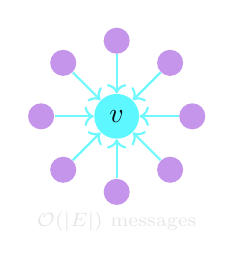
\begin{tikzpicture}[scale=0.6]
                \node[circle, fill=cyanneon!80, minimum size=0.5cm, text=darkbg, font=\bfseries] (v) at (0,0) {$v$};
                \foreach \i/\a in {1/45, 2/90, 3/135, 4/180, 5/225, 6/270, 7/315, 8/0} {
                    \node[circle, fill=violetelectric!60, minimum size=0.3cm] (n\i) at (\a:1.6) {};
                    \draw[->, thick, cyanneon!70] (n\i) -- (v);
                }
                \node[below=0.8cm of v, font=\scriptsize, text=lighttext] {$\mathcal{O}(|E|)$ messages};
            \end{tikzpicture}

            \vspace{0.3cm}
            {\scriptsize\textcolor{distillgrey}{[1] Kipf \& Welling, ICLR 2017}}
        \end{column}
    \end{columns}
\end{frame}

% =============================================================================
% SLIDE 3: Intuition -- Why Sparsify?
% =============================================================================
\begin{frame}{\faCut \quad The Intuition: Why Sparsify?}
    \textbf{\textcolor{cyanneon}{Key Observation:}} Many edges are \alert{redundant}
    
    \vspace{0.3cm}
    \begin{columns}[T]
        \begin{column}{0.5\textwidth}
            \textbf{\textcolor{violetelectric}{Example: Citation Network}}
            \begin{itemize}
                \item Two papers cite the same 50 references
                \item Highly \emph{overlapping} neighborhoods
                \item Messages carry \emph{duplicate} information
            \end{itemize}
            
            \vspace{0.2cm}
            \textbf{\textcolor{violetelectric}{Sparsification Goal:}}
            \begin{itemize}
                \item Build $G' = (V, E')$ with $|E'| \ll |E|$
                \item Preserve essential structural properties
            \end{itemize}
        \end{column}
        \begin{column}{0.45\textwidth}
            \centering
            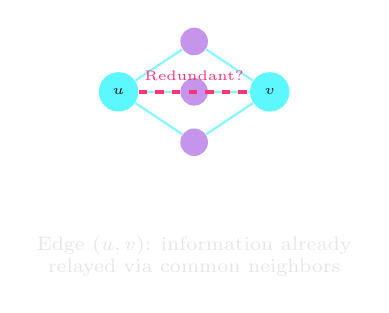
\begin{tikzpicture}[scale=0.8]
                % Two nodes with overlapping neighborhoods
                \node[circle, fill=cyanneon!80, minimum size=0.5cm, font=\tiny, text=darkbg] (u) at (-1.2, 0) {$u$};
                \node[circle, fill=cyanneon!80, minimum size=0.5cm, font=\tiny, text=darkbg] (v) at (1.2, 0) {$v$};
                
                % Shared neighbors
                \foreach \i/\y in {1/0.8, 2/0, 3/-0.8} {
                    \node[circle, fill=violetelectric!60, minimum size=0.35cm] (s\i) at (0, \y) {};
                    \draw[thick, cyanneon!60] (u) -- (s\i);
                    \draw[thick, cyanneon!60] (v) -- (s\i);
                }
                
                % Redundant edge
                \draw[ultra thick, magentaneon, dashed] (u) -- node[above, font=\tiny, text=magentaneon] {Redundant?} (v);
                
                \node[below=0.5cm, font=\scriptsize, align=center, text=lighttext] at (0, -1.5) {Edge $(u,v)$: information already\\relayed via common neighbors};
            \end{tikzpicture}
        \end{column}
    \end{columns}
\end{frame}

% =============================================================================
% SLIDE 4: Method 1 -- Metric Backbones (with MANIM-style diagram)
% =============================================================================
\begin{frame}[shrink=3]{\faRoute \quad Method 1: Metric Backbones}
    \begin{columns}[T]
        \begin{column}{0.48\textwidth}
            \textbf{\textcolor{cyanneon}{Idea:}} Keep only edges on shortest paths

            \vspace{0.15cm}
            \begin{exampleblock}{\faLightbulb \quad Definition}
                Edge $(u,v)$ is kept iff:
                \[
                w(u, v) = d_G(u, v)
                \]
            \end{exampleblock}

            \vspace{0.1cm}
            {\small\textcolor{lighttext}{If an indirect path is shorter $\Rightarrow$ edge is \alert{removed}}}

            \vspace{0.15cm}
            {\scriptsize\textcolor{distillgrey}{[4] Dreveton et al., NeurIPS 2024}}
        \end{column}
        \begin{column}{0.5\textwidth}
            \centering
            % CONCEPT A: METRIC BACKBONE - Triangle Inequality
            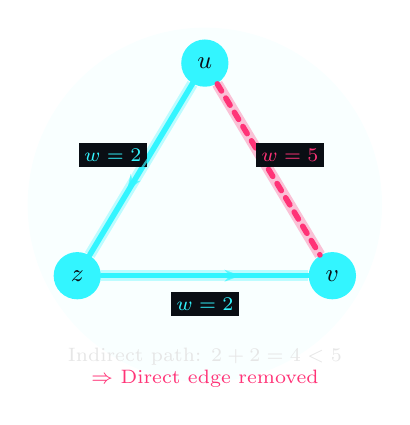
\begin{tikzpicture}[scale=0.9]
                % Background glow
                \fill[cyanneon, opacity=0.03] (0,0) circle (2.5cm);
                
                % Nodes with Manim-style glow
                \node[manim node, fill=cyanneon, text=darkbg] (A) at (0, 2) {$u$};
                \node[manim node, fill=cyanneon, text=darkbg] (B) at (-1.8, -1) {$z$};
                \node[manim node, fill=cyanneon, text=darkbg] (C) at (1.8, -1) {$v$};
                
                % Direct edge (REMOVED - heavy, magenta)
                \draw[manim glow, magentaneon] (A) -- (C);
                \draw[manim edge, magentaneon, dashed] (A) -- (C);
                \node[font=\scriptsize, text=magentaneon, fill=darkbg, inner sep=2pt] at (1.2, 0.7) {$w=5$};
                
                % Indirect path (KEPT - light, cyan)
                \draw[manim glow, cyanneon] (A) -- (B);
                \draw[manim edge, cyanneon] (A) -- (B);
                \node[font=\scriptsize, text=cyanneon, fill=darkbg, inner sep=2pt] at (-1.3, 0.7) {$w=2$};
                
                \draw[manim glow, cyanneon] (B) -- (C);
                \draw[manim edge, cyanneon] (B) -- (C);
                \node[font=\scriptsize, text=cyanneon, fill=darkbg, inner sep=2pt] at (0, -1.4) {$w=2$};
                
                % Annotation
                \node[font=\scriptsize, text=lighttext, align=center] at (0, -2.3) {
                    Indirect path: $2+2=4 < 5$\\
                    \textcolor{magentaneon}{$\Rightarrow$ Direct edge removed}
                };
                
                % Flow arrows
                \draw[-{Stealth[length=2mm]}, cyanneon, thick, opacity=0.7] (-0.7, 0.8) -- (-1.1, 0.2);
                \draw[-{Stealth[length=2mm]}, cyanneon, thick, opacity=0.7] (-0.5, -1) -- (0.5, -1);
            \end{tikzpicture}
        \end{column}
    \end{columns}
\end{frame}

% =============================================================================
% SLIDE 5: Jaccard vs Adamic-Adar (with MANIM-style diagram)
% =============================================================================
\begin{frame}[shrink=12]{\faBalanceScale \quad Jaccard vs Adamic-Adar: Which to Choose?}
    \begin{columns}[T]
        \begin{column}{0.55\textwidth}
            % CONCEPT B: HUB vs COMMUNITY NEIGHBOR
            \centering
            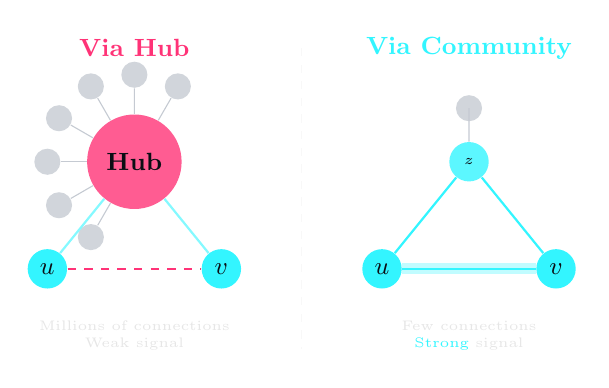
\begin{tikzpicture}[scale=0.85]
                % === LEFT SIDE: Sharing a HUB (bad signal) ===
                \node[font=\small\bfseries, text=magentaneon] at (-2.5, 2.5) {Via Hub};
                
                % Hub node (large, magenta)
                \node[circle, minimum size=1.2cm, fill=magentaneon!80, text=darkbg, font=\small\bfseries] (hub) at (-2.5, 0.8) {Hub};
                
                % Many connections to hub
                \foreach \a in {60, 90, 120, 150, 180, 210, 240} {
                    \node[circle, fill=distillgrey!40, minimum size=0.2cm] (h\a) at ($(-2.5, 0.8) + (\a:1.3)$) {};
                    \draw[distillgrey!50, thin] (hub) -- (h\a);
                }
                
                % Our two nodes
                \node[manim node, fill=cyanneon, text=darkbg, minimum size=0.5cm] (u1) at (-3.8, -0.8) {$u$};
                \node[manim node, fill=cyanneon, text=darkbg, minimum size=0.5cm] (v1) at (-1.2, -0.8) {$v$};
                
                \draw[thick, cyanneon!60] (u1) -- (hub);
                \draw[thick, cyanneon!60] (v1) -- (hub);
                \draw[thick, magentaneon, dashed] (u1) -- (v1);
                
                \node[font=\tiny, text=lighttext, align=center] at (-2.5, -1.8) {Millions of connections\\\alert{Weak} signal};
                
                % === RIGHT SIDE: Sharing a COMMUNITY node (good signal) ===
                \node[font=\small\bfseries, text=cyanneon] at (2.5, 2.5) {Via Community};
                
                % Small community node
                \node[circle, minimum size=0.5cm, fill=cyanneon!80, text=darkbg, font=\tiny\bfseries] (comm) at (2.5, 0.8) {$z$};
                
                % Few connections
                \node[circle, fill=distillgrey!40, minimum size=0.15cm] at ($(comm) + (90:0.8)$) {};
                \draw[distillgrey!50, thin] (comm) -- ++(90:0.8);
                
                % Our two nodes
                \node[manim node, fill=cyanneon, text=darkbg, minimum size=0.5cm] (u2) at (1.2, -0.8) {$u$};
                \node[manim node, fill=cyanneon, text=darkbg, minimum size=0.5cm] (v2) at (3.8, -0.8) {$v$};
                
                \draw[thick, cyanneon] (u2) -- (comm);
                \draw[thick, cyanneon] (v2) -- (comm);
                \draw[thick, cyanneon] (u2) -- (v2);
                
                % Glow effect
                \draw[cyanneon, opacity=0.3, line width=4pt] (u2) -- (v2);
                
                \node[font=\tiny, text=lighttext, align=center] at (2.5, -1.8) {Few connections\\\textcolor{cyanneon}{Strong} signal};
                
                % Divider
                \draw[lighttext!30, dashed] (0, 2.5) -- (0, -2);
            \end{tikzpicture}
        \end{column}
        \begin{column}{0.42\textwidth}
            \textbf{\textcolor{cyanneon}{\faFile \quad Jaccard Similarity}}
            \vspace{-0.1cm}
            \[
            J(u,v) = \frac{|N(u) \cap N(v)|}{|N(u) \cup N(v)|}
            \]
            \vspace{-0.2cm}
            \begin{itemize}\setlength{\itemsep}{0pt}
                \item Treats all neighbors \emph{equally}
                \item Homogeneous degrees (rather rare)
            \end{itemize}

            \vspace{0.15cm}
            \textbf{\textcolor{magentaneon}{\faUsers \quad Adamic-Adar Index}}
            \vspace{-0.1cm}
            \[
            \mathrm{AA}(u,v) = \!\!\sum_{z \in N(u) \cap N(v)} \frac{1}{\log |N(z)|}
            \]
            \vspace{-0.2cm}
            \begin{itemize}\setlength{\itemsep}{0pt}
                \item \alert{Penalizes} high-degree hubs
                \item $\Rightarrow$ \textbf{Social networks}
            \end{itemize}

            \vspace{0.1cm}
            {\footnotesize\textcolor{goldaccent}{Both are \textbf{similarities}} -- transform to dissimilarity for backbone: $w = 1/J$ or $w = 1/(1+\mathrm{AA})$}

            \vspace{0.05cm}
            {\scriptsize\textcolor{distillgrey}{[7] Adamic \& Adar, 2003}}
        \end{column}
    \end{columns}
\end{frame}

% =============================================================================
% SLIDE 6: Method 2 -- Spectral Sparsification (with ANIMATION)
% =============================================================================
\begin{frame}[shrink=5]{\faWaveSquare \quad Method 2: Spectral Sparsification}
    \begin{columns}[T]
        \begin{column}{0.52\textwidth}
            \textbf{\textcolor{cyanneon}{Idea:}} Preserve spectral properties of the Laplacian

            \begin{exampleblock}{\faLightbulb \quad Effective Resistance}
                \[
                R_{\text{eff}}(u,v) = L^+_{uu} + L^+_{vv} - 2L^+_{uv}
                \]
                {\small $L^+$: \textbf{pseudoinverse} of graph Laplacian $L = D - A$}
            \end{exampleblock}

            \vspace{0.1cm}
            \textbf{\textcolor{cyanneon}{\faBolt \quad Electrical Analogy:}}
            \begin{itemize}\setlength{\itemsep}{0pt}
                \item \textbf{High} $R_{\text{eff}}$: ``bridge'' (few alternative paths)
                \item \textbf{Low} $R_{\text{eff}}$: redundant (many parallel paths)
            \end{itemize}

            \vspace{0.1cm}
            \begin{alertblock}{\faBolt \quad Sampling Rule}
                Keep edge $e$ with prob.\ $p_e = w_e \cdot R_{\text{eff}}(e)$\\
                If kept, \textbf{reweight} to $1 / R_{\text{eff}}(e)$
            \end{alertblock}
            {\scriptsize\textcolor{distillgrey}{[2] Spielman \& Srivastava, STOC 2008}}
        \end{column}
        \begin{column}{0.46\textwidth}
            \centering
            % =================================================================
            % ANIMATED LAPLACIAN VISUALIZATION
            % Requires: laplacian_frames/frame_0.png to frame_30.png
            % =================================================================
            % If animation frames exist, use:
            % \animategraphics[loop, autoplay, width=0.95\textwidth]{10}{laplacian_frames/frame_}{0}{30}
            
            % Fallback static diagram (CONCEPT C: Effective Resistance)
            \begin{tikzpicture}[scale=0.8]
                % Background
                \fill[subtleglow, rounded corners] (-2.8, -2.3) rectangle (2.8, 2.5);
                
                % Title
                \node[font=\scriptsize\bfseries, text=cyanneon] at (0, 2.2) {Equivalent Circuit};
                
                % Two communities
                \fill[cyanneon, opacity=0.1, rounded corners=8pt] (-2.5, -1.8) rectangle (-0.3, 1.5);
                \fill[cyanneon, opacity=0.1, rounded corners=8pt] (0.3, -1.8) rectangle (2.5, 1.5);
                
                % Community A nodes
                \node[manim node, fill=cyanneon, text=darkbg, minimum size=0.4cm] (a1) at (-1.8, 0.8) {};
                \node[manim node, fill=cyanneon, text=darkbg, minimum size=0.4cm] (a2) at (-0.8, 0.8) {};
                \node[manim node, fill=cyanneon, text=darkbg, minimum size=0.4cm] (a3) at (-1.3, -0.2) {};
                \node[manim node, fill=cyanneon, text=darkbg, minimum size=0.4cm] (a4) at (-1.8, -1.2) {};
                \node[manim node, fill=cyanneon, text=darkbg, minimum size=0.4cm] (a5) at (-0.8, -1.2) {};
                
                % Community A internal edges
                \foreach \x/\y in {a1/a2, a1/a3, a2/a3, a3/a4, a3/a5, a4/a5} {
                    \draw[cyanneon!50, thin] (\x) -- (\y);
                }
                
                % Community B nodes
                \node[manim node, fill=cyanneon, text=darkbg, minimum size=0.4cm] (b1) at (0.8, 0.8) {};
                \node[manim node, fill=cyanneon, text=darkbg, minimum size=0.4cm] (b2) at (1.8, 0.8) {};
                \node[manim node, fill=cyanneon, text=darkbg, minimum size=0.4cm] (b3) at (1.3, -0.2) {};
                \node[manim node, fill=cyanneon, text=darkbg, minimum size=0.4cm] (b4) at (0.8, -1.2) {};
                \node[manim node, fill=cyanneon, text=darkbg, minimum size=0.4cm] (b5) at (1.8, -1.2) {};
                
                % Community B internal edges
                \foreach \x/\y in {b1/b2, b1/b3, b2/b3, b3/b4, b3/b5, b4/b5} {
                    \draw[cyanneon!50, thin] (\x) -- (\y);
                }
                
                % BRIDGE EDGE (HIGH RESISTANCE)
                \draw[manim glow, flowcolor] (a2) -- (b1);
                \draw[manim edge, flowcolor, flow arrow] (a2) -- (b1);
                
                % Flow particles
                \foreach \p in {0.2, 0.4, 0.6, 0.8} {
                    \node[circle, fill=flowcolor, minimum size=2pt, opacity=0.8] at ($(a2)!\p!(b1)$) {};
                }
                
                % Labels
                \node[font=\tiny, text=lighttext] at (-1.3, 1.3) {Cluster A};
                \node[font=\tiny, text=lighttext] at (1.3, 1.3) {Cluster B};
                
                % Resistance annotations
                \node[font=\tiny, text=flowcolor, fill=darkbg, inner sep=2pt, rounded corners] at (0, 1.0) {High $R_{\text{eff}}$};
                \node[font=\tiny, text=cyanneon!70, fill=darkbg, inner sep=1pt] at (-1.3, -1.7) {Low $R$};
                \node[font=\tiny, text=cyanneon!70, fill=darkbg, inner sep=1pt] at (1.3, -1.7) {Low $R$};
                
                % Current indicator
                \node[font=\tiny, text=flowcolor] at (0, -2.1) {\faBolt\ Critical flow};
            \end{tikzpicture}
        \end{column}
    \end{columns}
\end{frame}

% SLIDE 7: Removed (Graph Laplacian Energy Analogy -- not needed for 10min talk)

% =============================================================================
% SLIDE 8: Research Questions
% =============================================================================
\begin{frame}{\faSearch \quad Research Questions}
    \begin{enumerate}\setlength{\itemsep}{6pt}
        \item \textbf{\textcolor{cyanneon}{Accuracy--sparsity trade-off.}} Which sparsification strategies best preserve GNN accuracy as sparsity increases? Is there a saturation threshold?
        \item \textbf{\textcolor{cyanneon}{Computational efficiency.}} How does each method affect end-to-end training time (preprocessing + per-epoch cost)?
        \item \textbf{\textcolor{cyanneon}{Dataset dependence.}} Do citation vs.\ social graphs respond differently to metric vs.\ spectral sparsification?
        \item \textbf{\textcolor{cyanneon}{Ablation.}} Can we disentangle the effect of topology reduction from edge reweighting?
    \end{enumerate}
\end{frame}

% =============================================================================
% SLIDE 9: Experimental Pipeline
% =============================================================================
\begin{frame}{\faProjectDiagram \quad Experimental Pipeline}
    \centering
    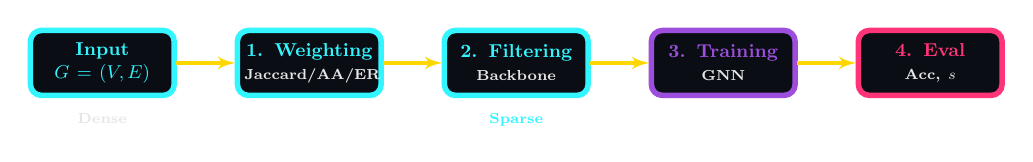
\begin{tikzpicture}[scale=0.75, transform shape, node distance=1.0cm, auto,
        block/.style={rectangle, draw=cyanneon, fill=darkbg, text=cyanneon, text width=2.2cm, text centered, rounded corners, minimum height=1.1cm, font=\small\bfseries, line width=2pt},
        line/.style={draw, -latex', very thick, goldaccent}]

        % Nodes - with high contrast colors
        \node [block] (input) {Input\\$G=(V, E)$};
        \node [block, right=of input] (weights) {1. Weighting\\{\scriptsize\textcolor{lighttext}{Jaccard/AA/ER}}};
        \node [block, right=of weights] (filter) {2. Filtering\\{\scriptsize\textcolor{lighttext}{Backbone}}};
        \node [block, right=of filter, draw=violetelectric, text=violetelectric] (gnn) {3. Training\\{\scriptsize\textcolor{lighttext}{GNN}}};
        \node [block, right=of gnn, draw=magentaneon, text=magentaneon] (eval) {4. Eval\\{\scriptsize\textcolor{lighttext}{Acc, $s$}}};

        % Arrows - gold for visibility
        \path [line] (input) -- (weights);
        \path [line] (weights) -- (filter);
        \path [line] (filter) -- (gnn);
        \path [line] (gnn) -- (eval);

        % Labels - brighter colors
        \node [below=0.15cm of input, text=lighttext, font=\scriptsize\bfseries] {Dense};
        \node [below=0.15cm of filter, text=cyanneon, font=\scriptsize\bfseries] {Sparse};
    \end{tikzpicture}
    
    \vspace{0.4cm}
    \begin{columns}[T]
        \begin{column}{0.48\textwidth}
            \centering
            \textbf{\textcolor{cyanneon}{\faDatabase \quad Datasets (12 benchmarks):}}
            \begin{itemize}\setlength{\itemsep}{0pt}
                \item Citation: Cora, CiteSeer, PubMed, DBLP, Cora\_ML
                \item WebKB: Cornell, Texas, Wisconsin
                \item Wikipedia: Chameleon, Squirrel
                \item Other: Actor, PPI
            \end{itemize}
        \end{column}
        \begin{column}{0.48\textwidth}
            \centering
            \textbf{\textcolor{violetelectric}{\faBrain \quad GNN Models:}}
            \begin{itemize}
                \item \textbf{GCN}: fixed aggregation
                \item \textbf{GraphSAGE}: no edge weights
                \item \textbf{GAT}: learned attention
            \end{itemize}
        \end{column}
    \end{columns}
\end{frame}

% =============================================================================
% SLIDE 9: Evaluation Metrics
% =============================================================================
\begin{frame}{\faChartBar \quad Evaluation Metrics}
    \begin{columns}[T]
        \begin{column}{0.48\textwidth}
            \centering
            \textbf{\textcolor{cyanneon}{\faTrophy \quad Performance:}}
            \begin{itemize}
                \item \textbf{Accuracy} on test set
                \item \textbf{Accuracy drop}: $\Delta = \text{Acc}(G) - \text{Acc}(G')$
                \item Averaged over 3 seeds
            \end{itemize}
            
            \vspace{0.4cm}
            \textbf{\textcolor{violetelectric}{\faClock \quad Efficiency:}}
            \begin{itemize}
                \item \textbf{Sparsity ratio}: $s = |E'|/|E|$
                \item \textbf{Time}: preprocessing + training
            \end{itemize}
        \end{column}
        \begin{column}{0.48\textwidth}
            \centering
            \textbf{\textcolor{magentaneon}{\faBullseye \quad Objective:}}
            \begin{center}
                \alert{Maximize sparsity\\while minimizing $\Delta$}
            \end{center}

            \vspace{0.4cm}
            \textbf{\textcolor{violetelectric}{\faFlask \quad Ablation Design:}}
            \begin{itemize}
                \item Disentangle topology reduction vs.\ edge reweighting
                \item 4 scenarios $\times$ 3 seeds
            \end{itemize}
        \end{column}
    \end{columns}
\end{frame}

% =============================================================================
% SLIDE 10: Ablation Study (A/B/C/D)
% =============================================================================
\begin{frame}[shrink=3]{\faFlask \quad Ablation Study: Disentangling Effects}
    \textbf{\textcolor{cyanneon}{Question:}} Does improvement come from \alert{topology} or \alert{reweighting}?
    
    \vspace{0.1cm}
    \begin{center}\small
    \begin{tabular}{lcc}
        \toprule
        \textbf{\textcolor{lighttext}{Scenario}} & \textbf{\textcolor{lighttext}{Graph}} & \textbf{\textcolor{lighttext}{Weights}} \\
        \midrule
        \textbf{A} (baseline) & Complete & Binary \\
        \textbf{B} & \textcolor{cyanneon}{Sparse} & Binary \\
        \textbf{C} & Complete & \textcolor{violetelectric}{Learned} \\
        \textbf{D} & \textcolor{cyanneon}{Sparse} & \textcolor{violetelectric}{Learned} \\
        \bottomrule
    \end{tabular}
    \end{center}
    
    \vspace{0.1cm}
    \textbf{\textcolor{cyanneon}{\faSearchPlus \quad Interpreting Differences:}}
    \begin{itemize}\setlength{\itemsep}{0pt}
        \item $\mathbf{B - A}$ = \textbf{Structure effect} (edge removal alone)
        \item $\mathbf{C - A}$ = \textbf{Weighting effect} (reweighting alone)
        \item $\mathbf{D - A}$ = \textbf{Combined effect} (full sparsification)
    \end{itemize}
    {\scriptsize \textit{\textcolor{distillgrey}{Note: GraphSAGE doesn't support weights $\Rightarrow$ C = A and D = B}}}
\end{frame}

% =============================================================================
% SLIDE 11b: Preliminary Results -- Heatmap
% =============================================================================
\begin{frame}[shrink=5]{\faChartLine \quad Preliminary Results: Accuracy Heatmap (Cora)}
    \begin{columns}[T]
        \begin{column}{0.52\textwidth}
            \centering
            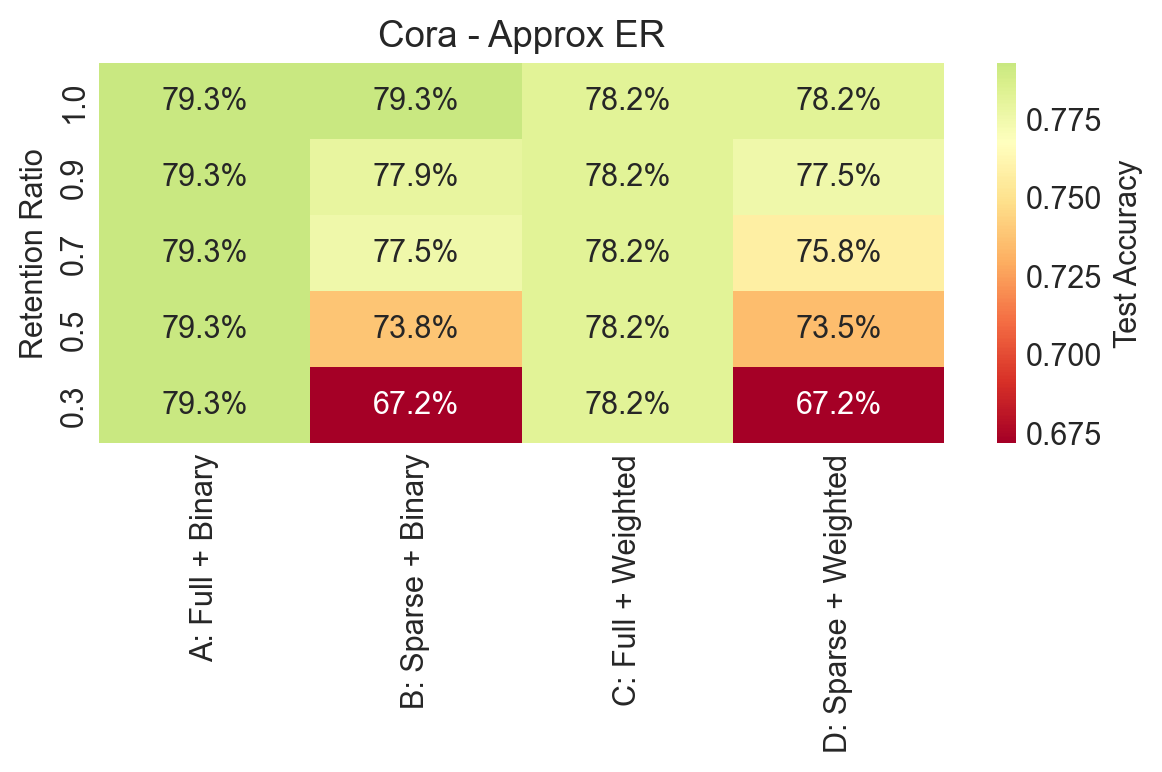
\includegraphics[width=\textwidth]{figures/heatmap_cora_er.png}
        \end{column}
        \begin{column}{0.45\textwidth}
            \textbf{\textcolor{cyanneon}{\faBolt \quad Approx ER dominates:}}
            \begin{center}\footnotesize
            \begin{tabular}{lccc}
                \toprule
                & \textbf{Jacc.} & \textbf{AA} & \textbf{ER} \\
                \midrule
                Cora     & 73.8 & 73.3 & \textcolor{cyanneon}{\textbf{78.2}} \\
                CiteSeer & 65.1 & 64.7 & \textcolor{cyanneon}{\textbf{67.5}} \\
                PubMed   & 74.7 & 74.4 & \textcolor{cyanneon}{\textbf{78.0}} \\
                \bottomrule
            \end{tabular}
            \end{center}
            {\scriptsize GCN, Scenario D, Metric Backbone (\%)}

            \vspace{0.15cm}
            \textbf{\textcolor{violetelectric}{\faShieldAlt \quad GAT most robust:}}
            \begin{itemize}\setlength{\itemsep}{0pt}
                \item GAT: 75.3--78.7\% (narrow)
                \item GCN: 70.4--78.2\% (metric-sensitive)
            \end{itemize}
        \end{column}
    \end{columns}
\end{frame}

% =============================================================================
% SLIDE 11c: Preliminary Results -- Scenarios
% =============================================================================
\begin{frame}[shrink=5]{\faChartLine \quad Preliminary Results: Scenario Comparison (Cora)}
    \begin{columns}[T]
        \begin{column}{0.52\textwidth}
            \centering
            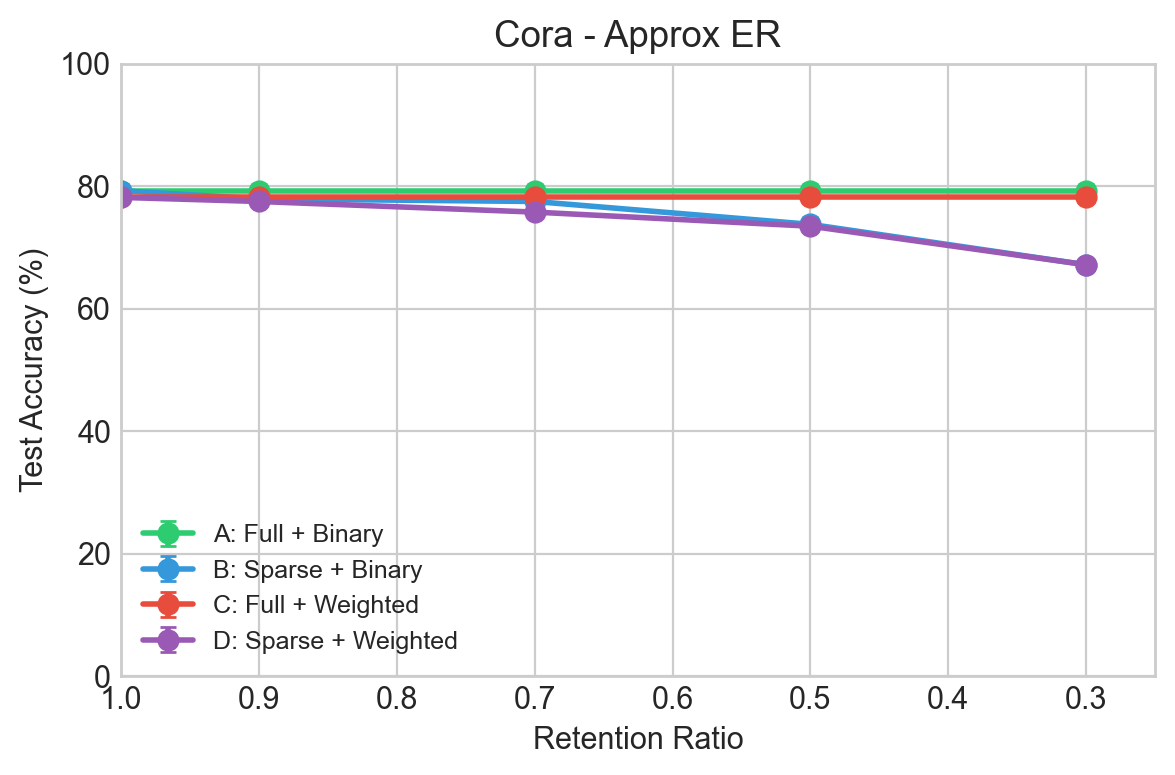
\includegraphics[width=\textwidth]{figures/scenarios_cora_er.png}
        \end{column}
        \begin{column}{0.45\textwidth}
            \textbf{\textcolor{magentaneon}{\faExclamationTriangle \quad Surprising:}}
            \begin{itemize}\setlength{\itemsep}{2pt}
                \item Backbone $\approx$ \textbf{no-op} on citations: retains \alert{99.5--99.9\%} of edges {\tiny\textcolor{goldaccent}{(similarity$\to$distance transform to verify)}}
                \item Weighting alone \textbf{hurts} ($-6.4$pp) but \textbf{synergy} with sparsification ($+4.5$pp)
                \item Below 40\% retention: significant accuracy drop
            \end{itemize}

            \vspace{0.15cm}
            \begin{alertblock}{\faArrowRight \quad Implication}
                {\small Denser graphs (Squirrel, Actor) needed to truly test backbones}
            \end{alertblock}
        \end{column}
    \end{columns}
\end{frame}

% =============================================================================
% SLIDE 12: Methods Summary
% =============================================================================
\begin{frame}[shrink=3]{\faList \quad Methods Summary}
    \begin{center}
    \begin{tabular}{lccc}
        \toprule
        \textbf{\textcolor{lighttext}{Method}} & \textbf{\textcolor{lighttext}{Complexity}} & \textbf{\textcolor{lighttext}{Preserves}} & \textbf{\textcolor{lighttext}{Use Case}} \\
        \midrule
        Random & $\mathcal{O}(m)$ & Nothing & Baseline \\
        \textcolor{cyanneon}{Jaccard Backbone} & $\mathcal{O}(m \cdot \bar{d})$ & Metric & Citations \\
        \textcolor{cyanneon}{AA-Inspired} & $\mathcal{O}(m \cdot \bar{d})$ & Approx. metric & Social \\
        Spectral (exact) & $\mathcal{O}(n^3)$ & Spectrum & Theoretical \\
        Spectral (approx.) & $\mathcal{O}(m \log n)$ & Spectrum & Practical \\
        \bottomrule
    \end{tabular}
    \end{center}
    
    \vspace{0.2cm}
    \begin{exampleblock}{\faLightbulb \quad Central Hypothesis}
        \textbf{Metric backbones} offer a better accuracy/sparsity trade-off than spectral methods on community-structured graphs.
    \end{exampleblock}
\end{frame}

% =============================================================================
% SLIDE 12: Conclusion & Next Steps
% =============================================================================
\begin{frame}{\faFlagCheckered \quad Conclusion \& Next Steps}
    \textbf{\textcolor{cyanneon}{\faCheckCircle \quad What We Proposed:}}
    \begin{itemize}\setlength{\itemsep}{1pt}
        \item Comparative study: Metric backbones vs Spectral methods
        \item Pipeline on 12 datasets, 3 GNN architectures (GCN, SAGE, GAT)
        \item Ablation design to isolate topology vs weighting effects
    \end{itemize}
    
    \vspace{0.15cm}
    \textbf{\textcolor{violetelectric}{\faRocket \quad Next Steps:}}
    \begin{itemize}\setlength{\itemsep}{1pt}
        \item Analyze accuracy-sparsity trade-off by graph type
        \item Study impact on heterophilic graphs
        \item Explore integration with DropEdge (dynamic sparsification)
    \end{itemize}
    
    \vspace{0.2cm}
    \begin{center}
        \Large\textcolor{cyanneon}{\faQuestionCircle \quad Questions?}
    \end{center}
\end{frame}

\end{document}
